\chapter{Estructura}

\section{Diagrama general de la estructura}

      \begin{figure}[H]
    \centering
    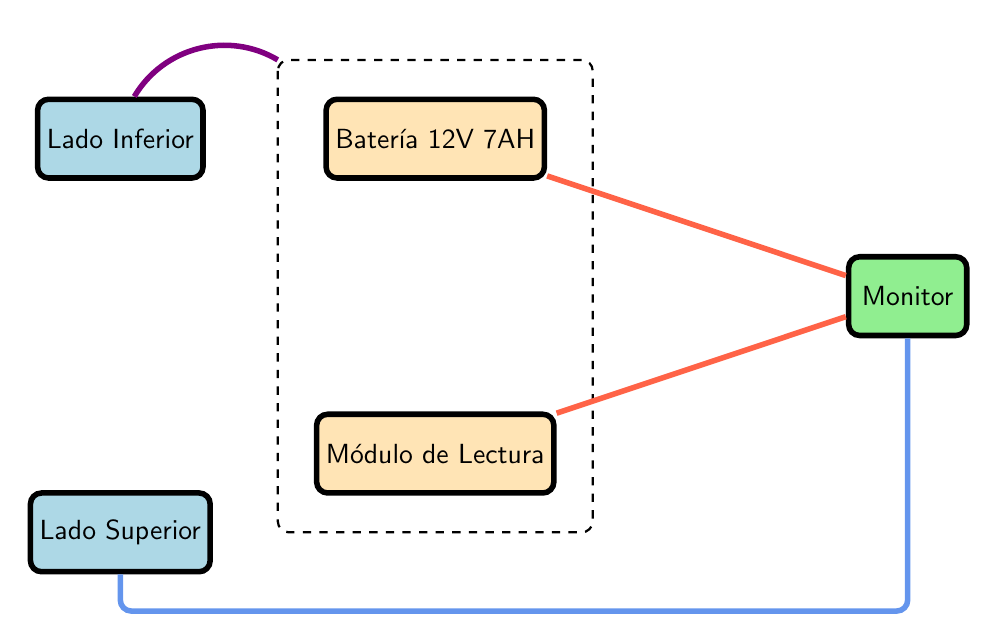
\begin{tikzpicture}[line width=2pt, rounded corners, every node/.style={font=\sffamily, draw, minimum width=1.5cm, minimum height=1cm, align=center}]
        
        % Colores personalizados
        \definecolor{colorEntrada}{RGB}{173, 216, 230} % Azul claro para entradas
        \definecolor{colorIntermedio}{RGB}{255, 228, 181} % Amarillo claro para nodos A y B
        \definecolor{colorSalida}{RGB}{144, 238, 144} % Verde claro para el nodo C
        
        % Colores para las flechas
        \definecolor{colorFlechaEntrada}{RGB}{100, 149, 237} % Azul para flechas de entrada
        \definecolor{colorFlechaIntermedio}{RGB}{255, 99, 71} % Rojo para flechas intermedias
        \definecolor{colorFlechaSalida}{RGB}{34, 139, 34} % Verde para flechas de salida
        \definecolor{colorFlechaMorada}{RGB}{128, 0, 128} % Morado para la flecha de entrada 1
        
        % Nodos (bloques) con las modificaciones
        \node[fill=colorEntrada] (entrada1) at (-4, 2) {Lado Inferior};
        \node[fill=colorEntrada] (entrada2) at (-4, -3) {Lado Superior};
        \node[fill=colorIntermedio] (A) at (0, 2) {Batería 12V 7AH}; % Batería más cerca
        \node[fill=colorIntermedio] (B) at (0, -2) {Módulo de Lectura}; % Módulo más cerca
        \node[fill=colorSalida] (C) at (6, 0) {Monitor};
        
        % Caja discontinua más grande en altura alrededor de A y B
        \draw[dashed, thick] (-2, 3) rectangle (2, -3); % Caja más grande
        
        % Conexiones con colores para las flechas, con mayor grosor
        \draw[color=colorFlechaMorada, line width=2pt, bend left=45] (entrada1) to (-2, 3); % Flecha morada curva
        \draw[color=colorFlechaEntrada, line width=2pt] (entrada2) -- ++(0, -1) -| (C); % Flecha de entrada 2 por abajo
        \draw[color=colorFlechaIntermedio, line width=2pt] (A) -- (C); % Flecha de A a C recta
        \draw[ color=colorFlechaIntermedio, line width=2pt] (B) -- (C); % Flecha de B a C recta
        
    \end{tikzpicture}
    \begin{center}
    \caption{Diagrama en bloques de la estructura de Rev-Control.}
    \label{fig:diagrama_bloques_estruc}
    \vspace{0.5cm} % Espacio entre el caption y la nota
    \small{Nota: El módulo de lectura está conectado al monitor mediante el cable RS232.}
    \end{center}
    \end{figure}


\section{Software de diseño utilizado}
    \noindent  % Evita el sangrado de la sección
        \begin{center}
            
\includegraphics[width=0.2\textwidth]{Imagenes/cinema-4d-logo.png}
            \captionof{figure}{Cinema4D}
            \label{fig:logo_cinema}
        \end{center}
    
    \noindent Cinema 4D es un software de modelado, animación y renderizado 3D desarrollado por Maxon. Es ampliamente utilizado en la industria del diseño gráfico, efectos visuales y producción de películas. Con su interfaz intuitiva y potentes herramientas, Cinema 4D permite a los diseñadores crear modelos 3D detallados, animaciones complejas, simulaciones de físicas realistas y efectos visuales de alta calidad. La capacidad de integrar con otros programas de diseño y su versatilidad lo convierten en una opción popular entre los profesionales de la animación y el modelado 3D.

\section{Descripción de cada parte de la estructura}

\begin{itemize}

    \item \textbf{Maletín:} Es una opción de almacenamiento robusta y resistente, ideal para transportar equipos y herramientas en condiciones exigentes. Fabricado con materiales de alta calidad, ofrece protección contra impactos, agua y polvo. Su diseño incluye cierres seguros, asas ergonómicas y una estructura interna personalizable para organizar el contenido. Las paredes internas estan hechas de madera y los bordes de aluminio.
    
    \item \textbf{Monitor KINSEAL:} El Kinseal AMZ070W01RAGD es una pantalla táctil HMI industrial de 7 pulgadas, diseñada para aplicaciones que requieren un rendimiento robusto. Soporta interfaces de comunicación como RS232, RS485 y RS422, y opera con un rango de voltaje DC de 10-30V. Su pantalla tiene una resolución de 800x480 y una luminosidad de 450 cd/m², con una pantalla táctil resistiva de 4 hilos. Además, cuenta con 128MB de almacenamiento SPI NAND y puertos USB para transferencia de datos y descarga de programas. Su panel frontal tiene clasificación IP65.
    
    \item \textbf{Módulo de lectura:} Aqui estan los circuitos, conexiones y el cerebro del proyecto, El LPC845, donde esta todo lo necesario para usar Rev-Control. El modulo de lectura usa de base una caja modelo  Estanca 6 - Codigo: CE6 (Medidas: 300x210x80).
    
    \item \textbf{Batería de 12V:} La batería de plomo ácido gel es una batería sellada de 12 voltios y 7.0 Ah (amperios-hora), diseñada para ofrecer una alta fiabilidad y rendimiento en aplicaciones de respaldo de energía y sistemas de seguridad. Utiliza tecnología de gel, lo que la hace más resistente a las vibraciones y evita fugas de ácido, lo que la hace más segura y duradera. Es ideal para dispositivos como UPS, alarmas, sistemas solares y otros equipos que requieren energía confiable y constante.
    
\end{itemize}



\section{Imágenes exportadas de los diseños}
    
    \begin{itemize}
        \item \textbf{Diseño de maletín:} Recreación del maletín estilo ambil para ilustración.
        \begin{center}
            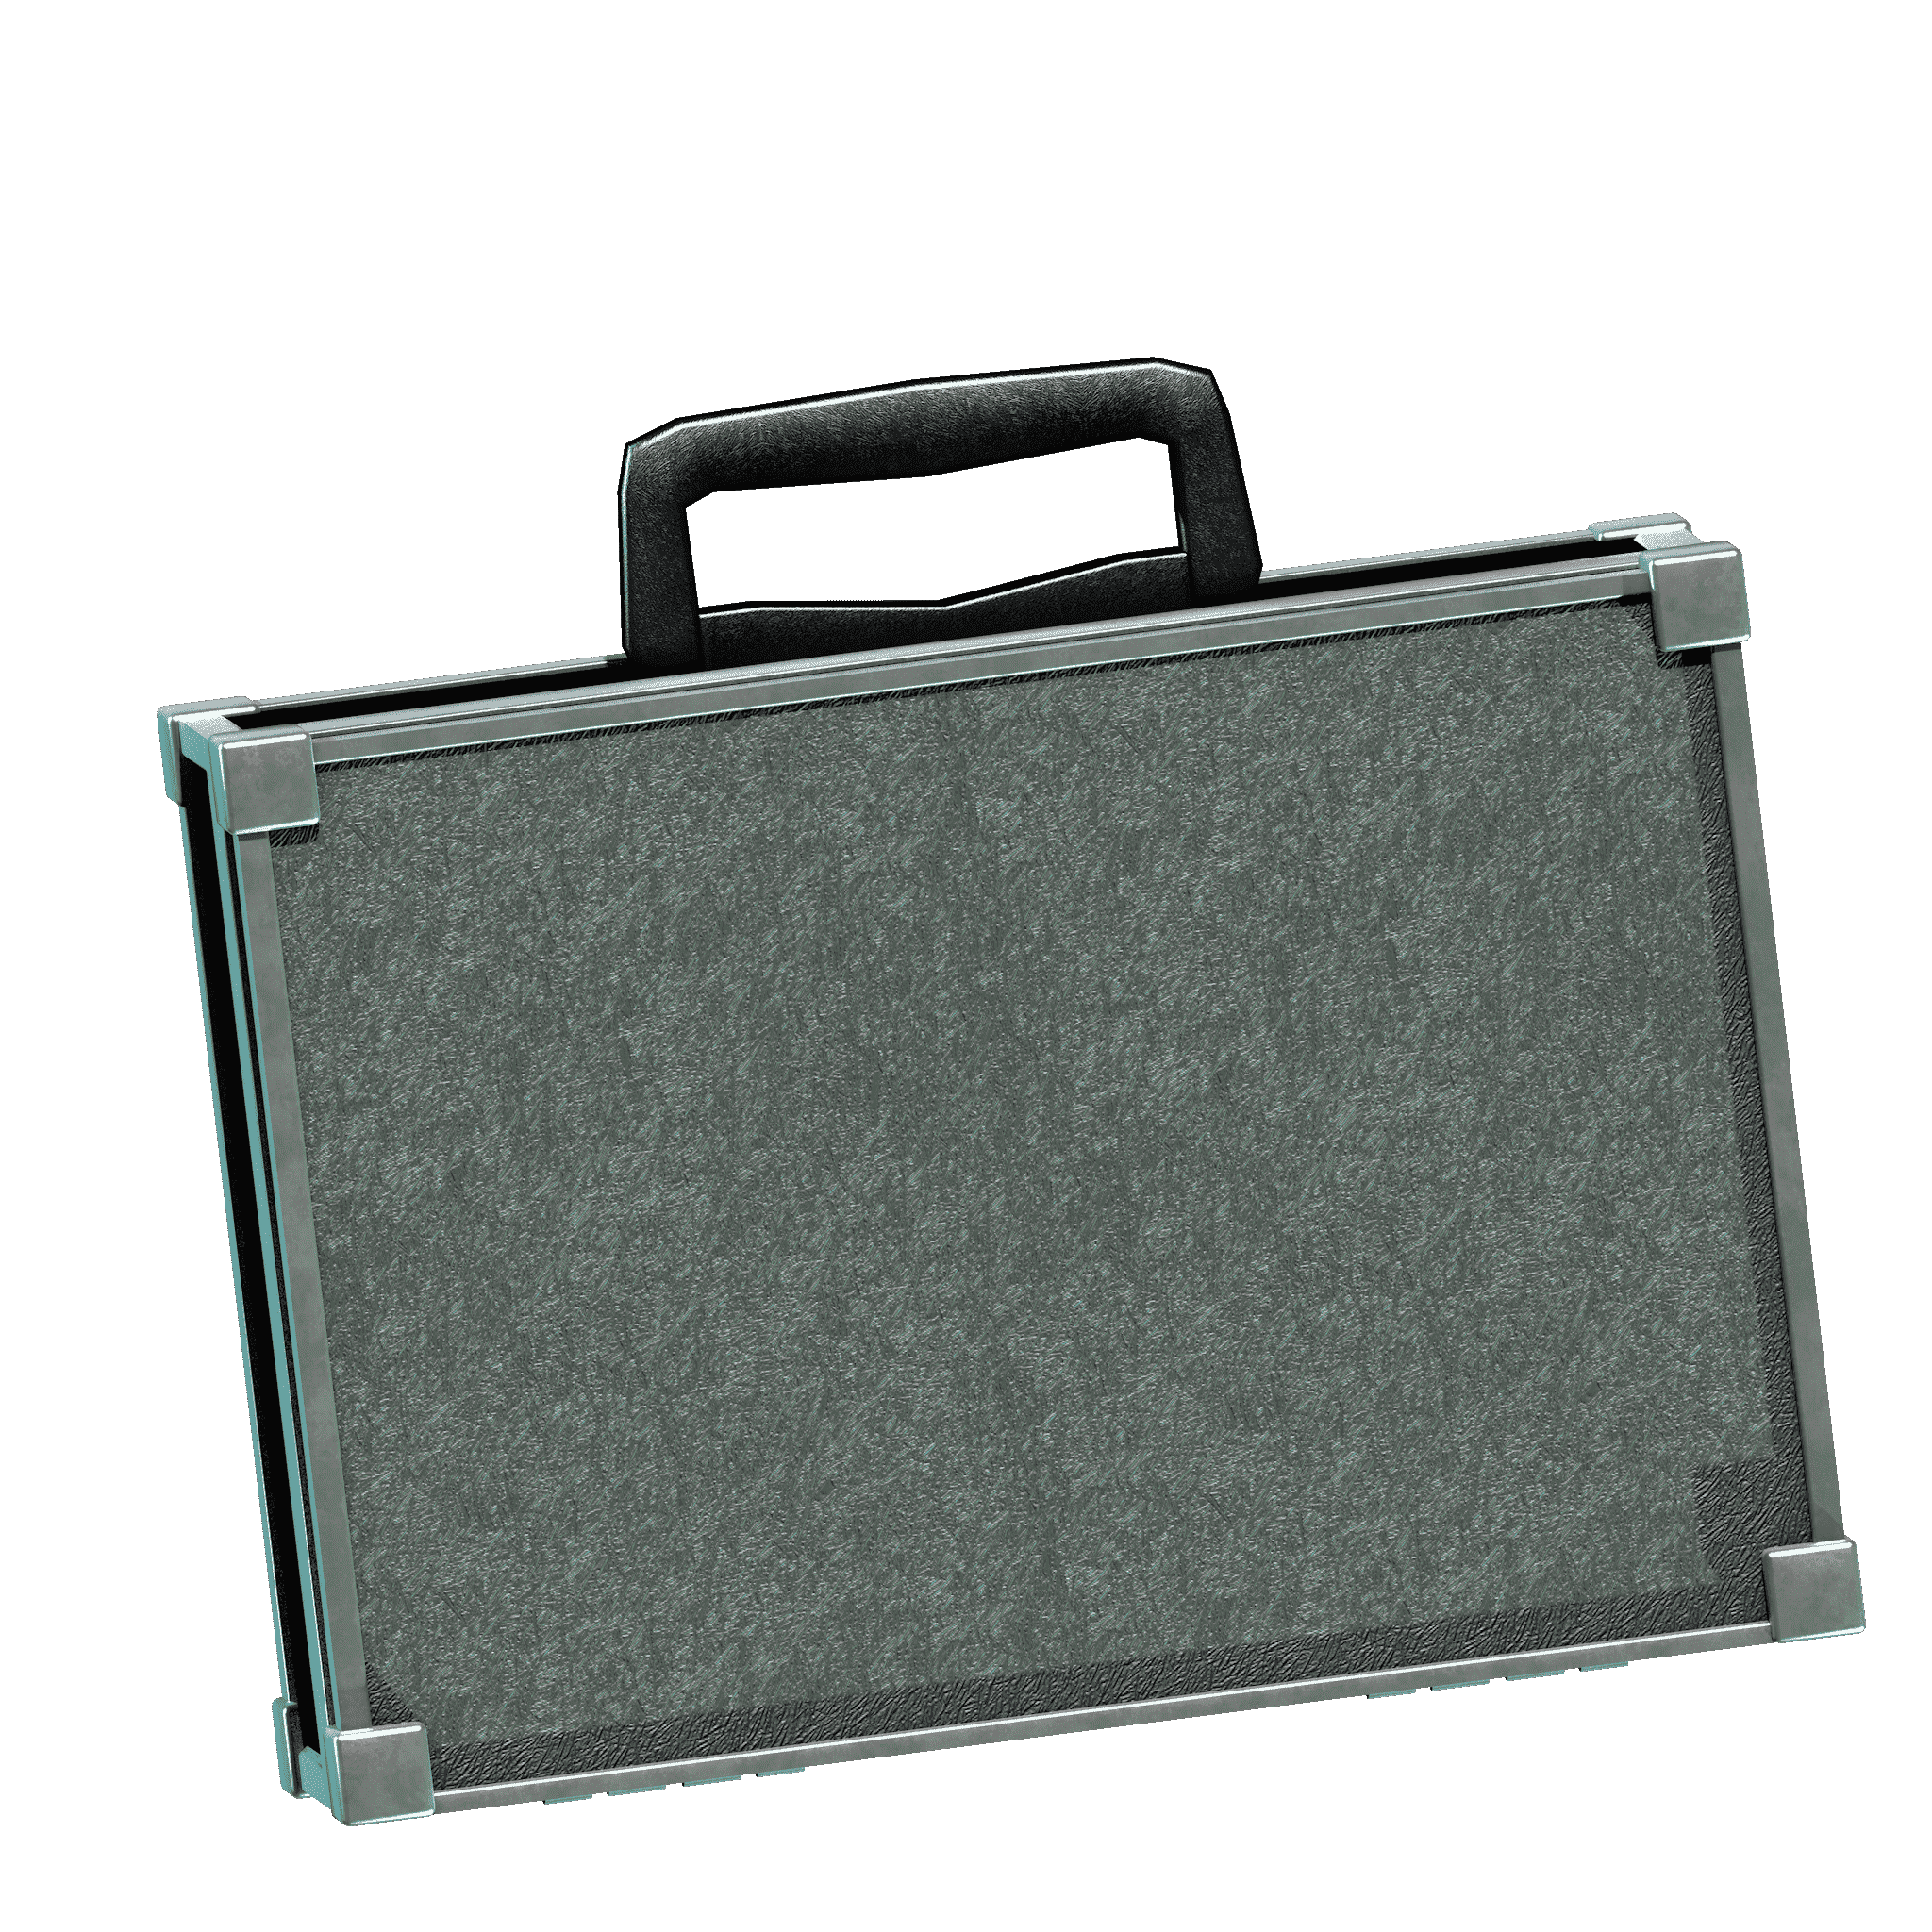
\includegraphics[width=0.8\textwidth]{Imagenes/Monitor y maletin42134.png}
            \captionof{figure}{Diseño de maletín}
            \label{fig:imagen1}
        \end{center}
        
        \item \textbf{Maletín abierto mostrando la interfaz digital:} Se usó un maletín estilo ambil para contener el módulo de lectura de datos y una batería de 12V 70Ah junto al monitor Kinseal en la tapa del maletín para visualizar su lectura.
        \begin{center}
            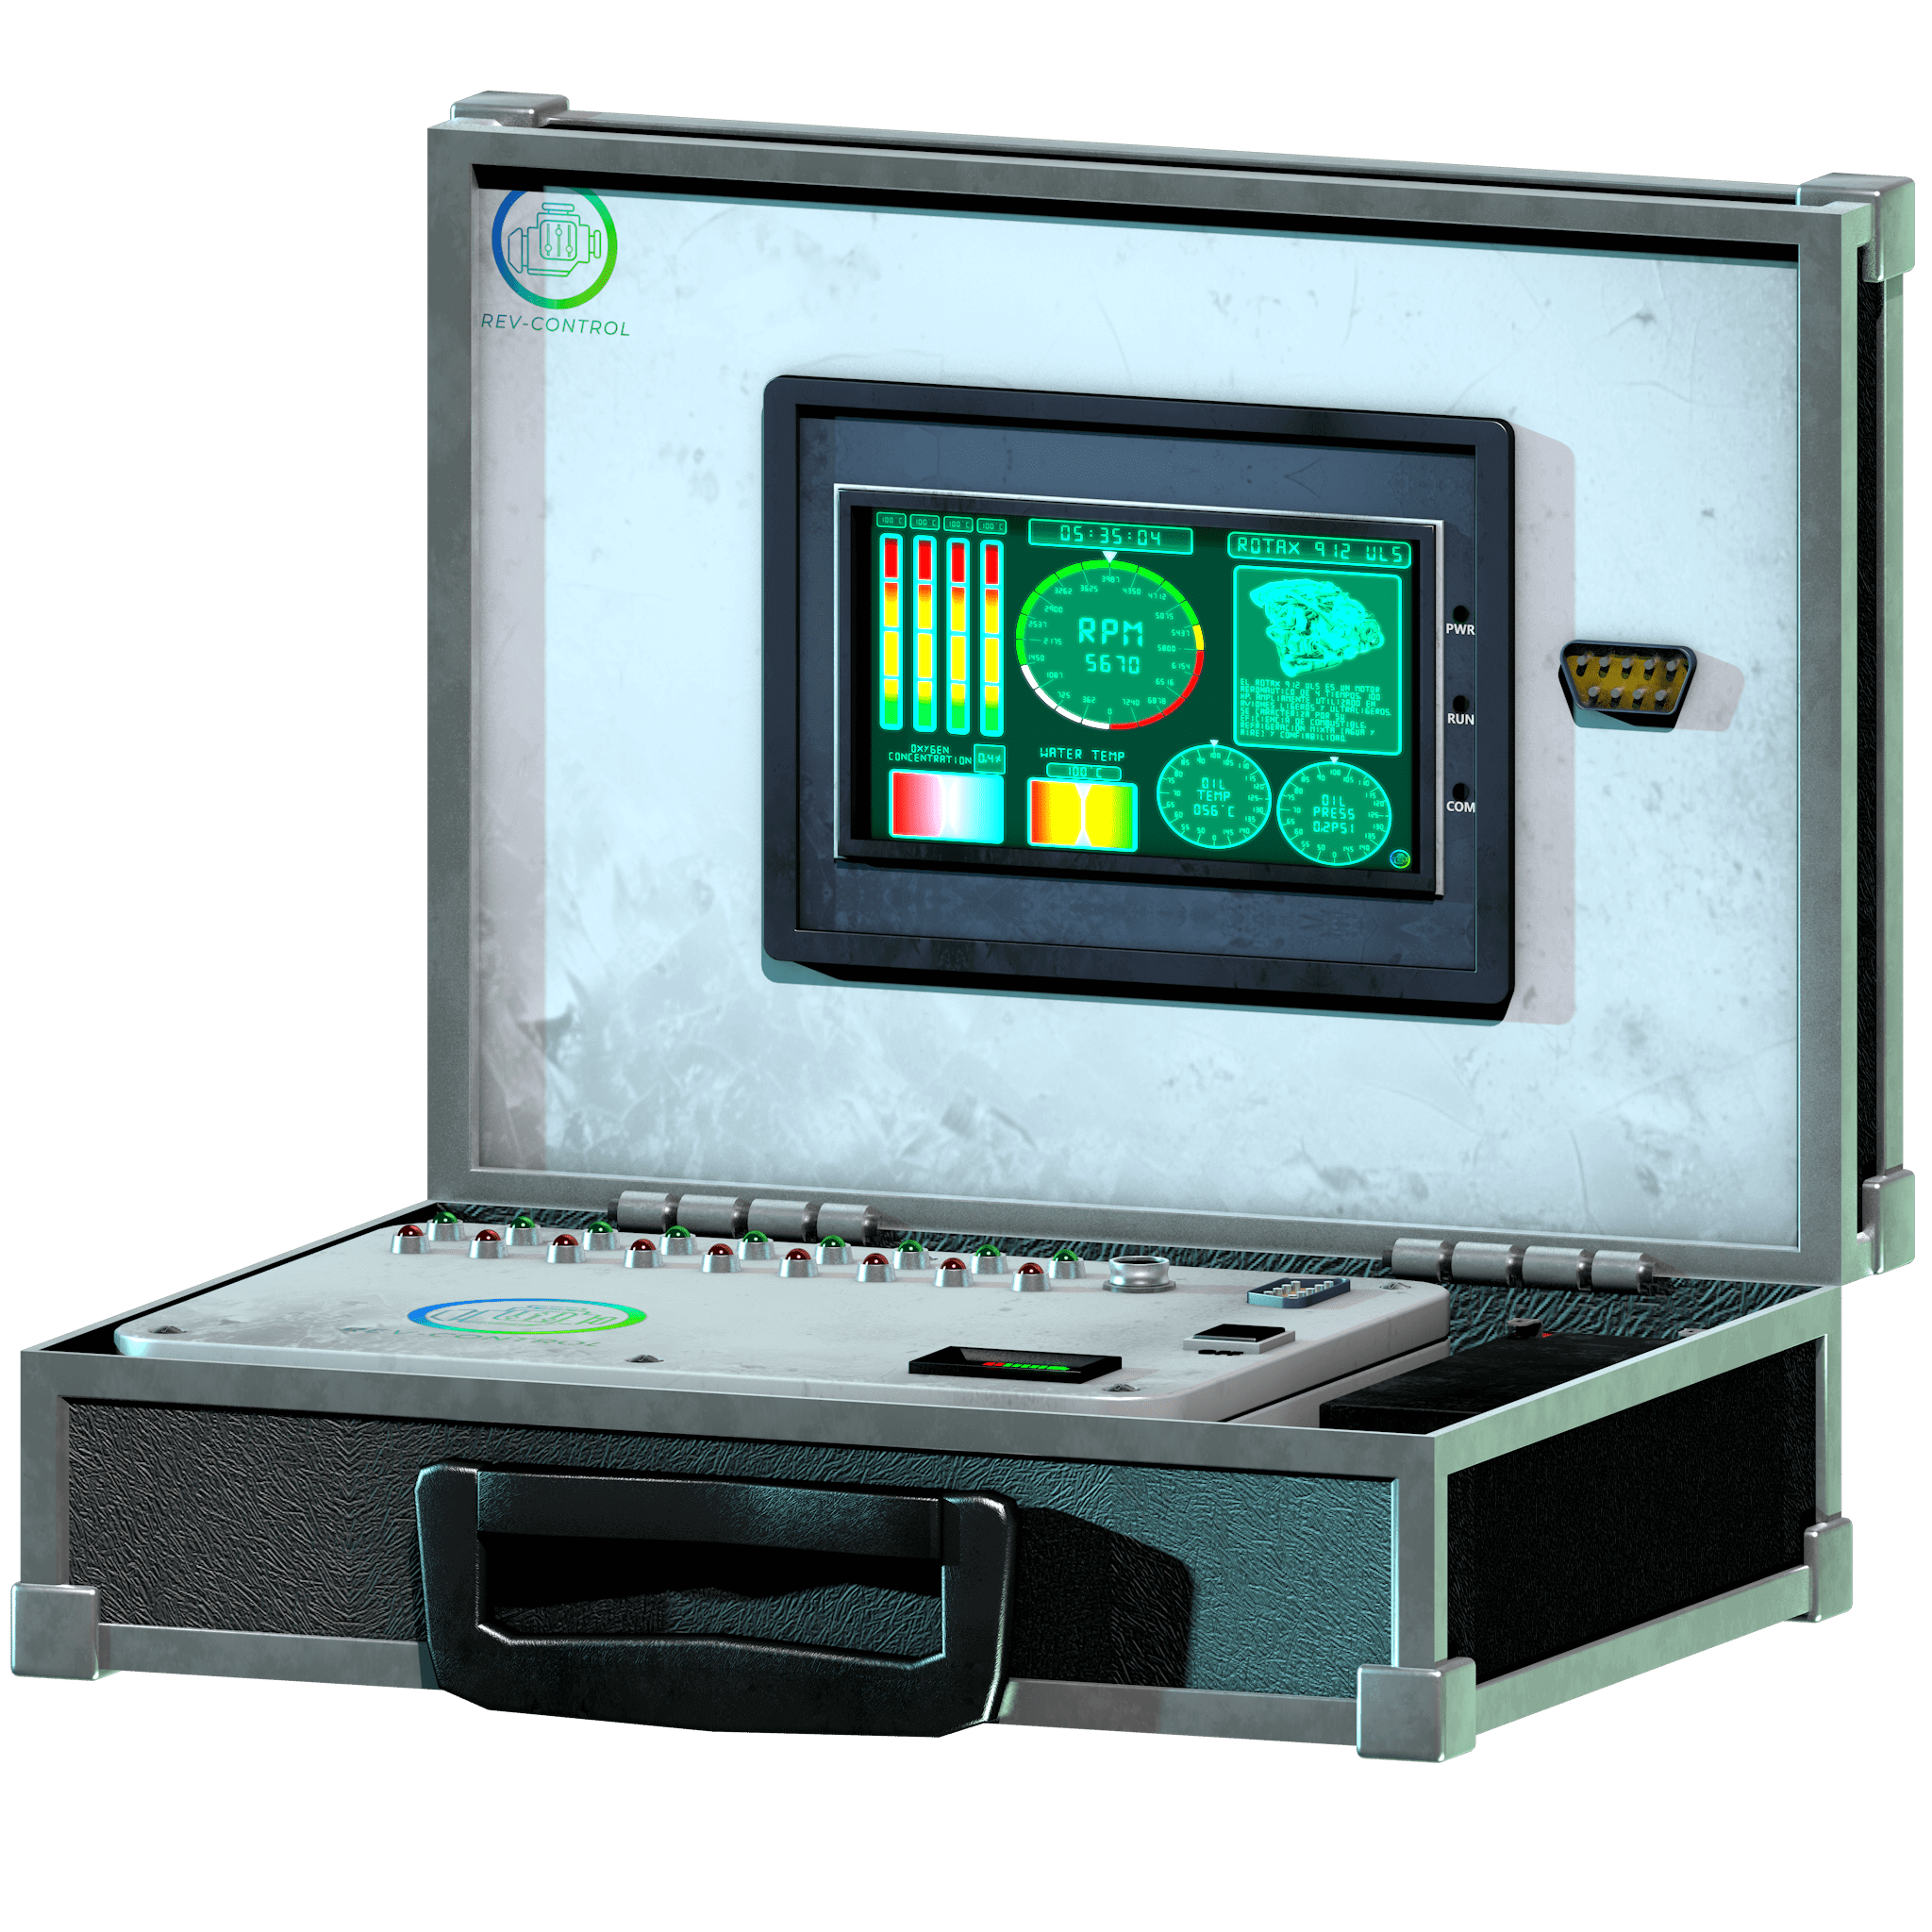
\includegraphics[width=0.8\textwidth]{Imagenes/Monitor y maletin-min.png}
            \captionof{figure}{Maletín abierto mostrando la interfaz digital}
            \label{fig:imagen2}
        \end{center}
        
        \item \textbf{Módulo de lectura de datos:} Este tiene las alarmas ojos de buey, un buzzer, un conector RS232, un switch de encendido, un voltímetro para mostrar la alimentación de la batería y atrás los conectores de cada sensor.
        \begin{center}
            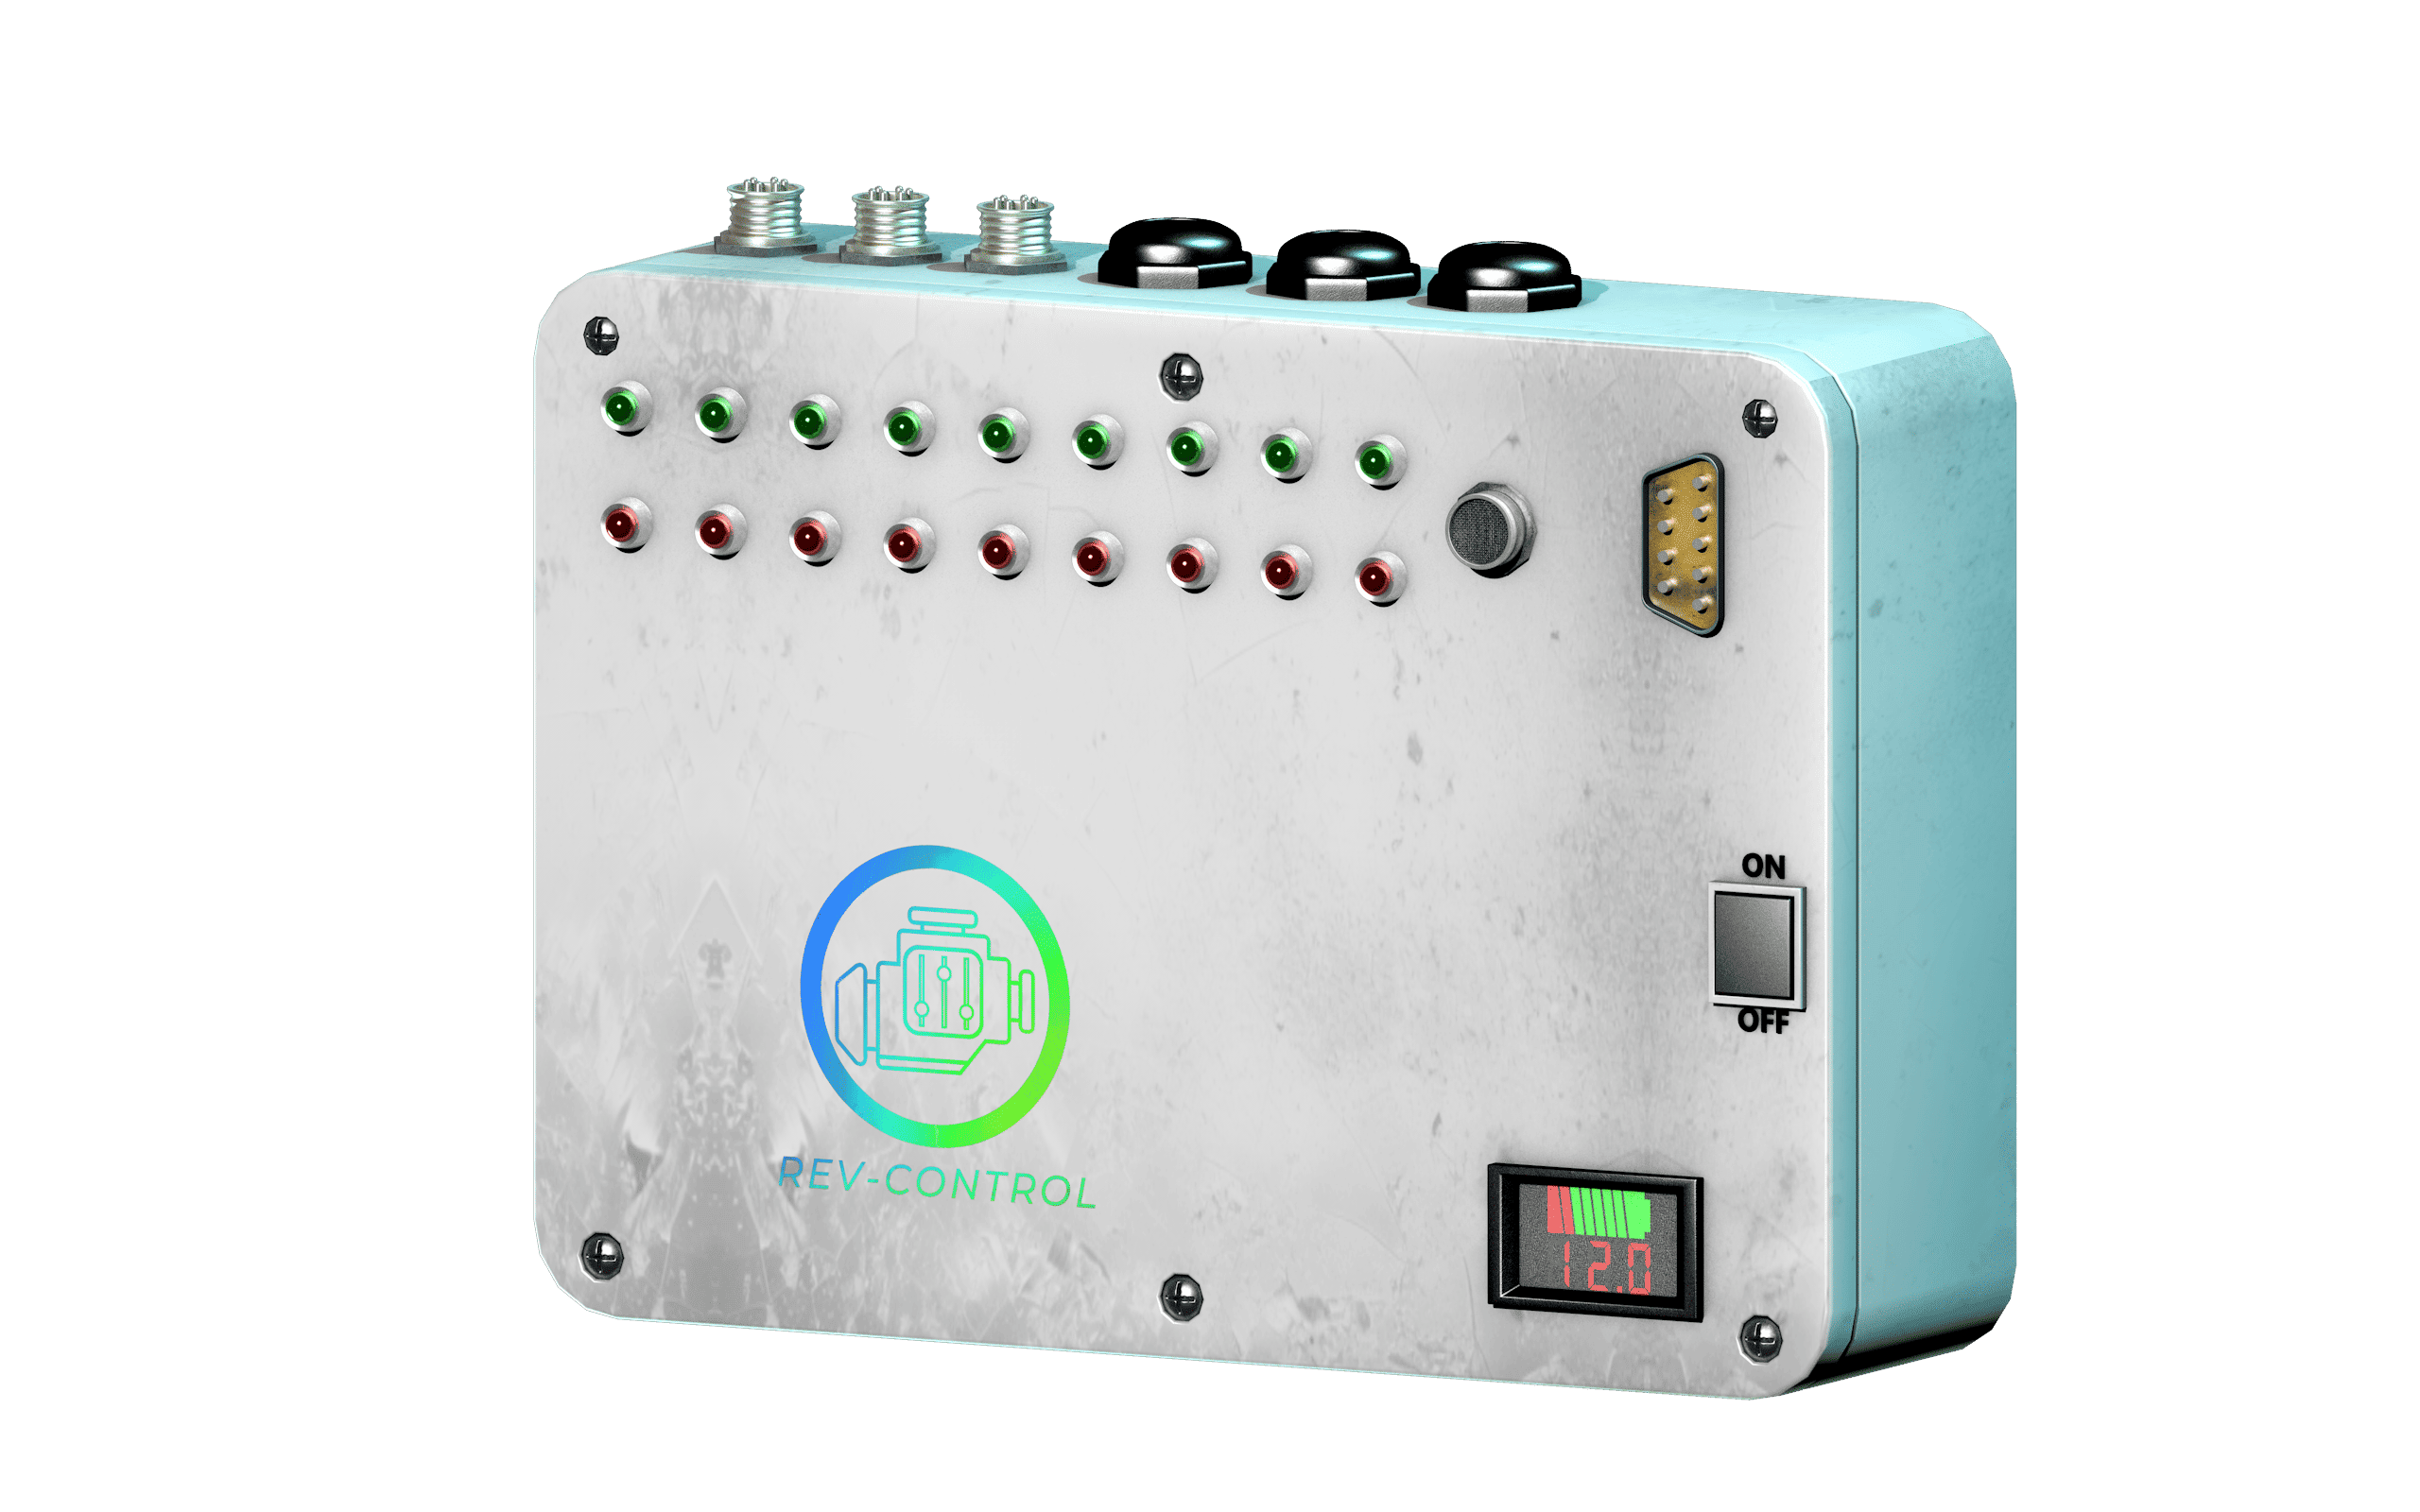
\includegraphics[width=0.8\textwidth]{Imagenes/Tablero rev control.png}
            \captionof{figure}{Módulo de lectura de datos}
            \label{fig:imagen3}
        \end{center}
    \end{itemize}
    
    